% Version 1

\documentclass[10pt]{llncs}

\usepackage{ucs}
\usepackage[utf8]{inputenc}
\usepackage{amsmath}
\usepackage{amsfonts}

\let\proof\relax
\let\endproof\relax

\usepackage{mathtools}
\usepackage{amsthm}
\usepackage{stmaryrd}
\usepackage{tikz}
\usetikzlibrary{calc}
\usepackage[noend]{algpseudocode}
\usepackage{algorithm}
\usepackage{xcolor}
\usepackage{graphicx}
\usepackage{multirow}
\usepackage{changepage}
\usepackage{todonotes}
\usepackage{comment}
\usepackage{blkarray}


\newcommand{\QQIF}[1] {\State \textbf{if} (#1)}
\newcommand{\QQRETURN} {\textbf{return} }

\title{The maximum grid contraction problem}
\author{
	Dimitri Watel\inst{1,2}
\and
	Pierre-Louis Poirion\inst{1,3}}
\institute{
 CEDRIC-CNAM, 292 rue du faubourg Saint Martin, 75003, Paris, FRANCE
\and
 ENSIIE, 1 Square de la résistance, Evry, FRANCE
  \email{dimitri.watel@ensiie.fr, }
\and
ENSTA Paristech
  \email{pierre-louis.poirion@ensta-paristech.fr}
}

\usepackage{caption}
\captionsetup[table]{aboveskip=5pt, }

\setcounter{secnumdepth}{3}


\newcommand{\gridsize}{0.5}
\newcommand{\prgrid}[3]{\draw[step=\gridsize,gray,very thin] (#1) grid (\gridsize*#3,\gridsize*#2);}
\newcommand{\prtline}[3]{}%\draw[] ($(#1)+(0,\gridsize*#2)$) -- ($(#1)+(\gridsize*#3,\gridsize*#2)$);}
\newcommand{\prtcolumn}[3]{}%\draw[] ($(#1)+(\gridsize*#2,0)$) -- ($(#1)+(\gridsize*#2,\gridsize*#3)$);}
\newcommand{\prvtline}[3]{\draw[very thick] ($(#1)+(0,\gridsize*#2)$) -- ($(#1)+(\gridsize*#3,\gridsize*#2)$);}
\newcommand{\prvtcolumn}[3]{\draw[very thick] ($(#1)+(\gridsize*#2,0)$) -- ($(#1)+(\gridsize*#2,\gridsize*#3)$);}
\newcommand{\prvtdline}[3]{\draw[very thick,dotted] ($(#1)+(0,\gridsize*#2)$) -- ($(#1)+(\gridsize*#3,\gridsize*#2)$);}
\newcommand{\prvtdcolumn}[3]{\draw[very thick,dotted] ($(#1)+(\gridsize*#2,0)$) -- ($(#1)+(\gridsize*#2,\gridsize*#3)$);}
\newcommand{\prbul}[3]{\draw ($(#1)+(#3*\gridsize-0.5*\gridsize,#2*\gridsize-0.5*\gridsize)$) node {$1$};}


\renewenvironment{comment}{\begingroup\sffamily\color{red} \itshape}{\endgroup}
\newcommand{\transpose}[1]{\ensuremath{#1^{\scriptscriptstyle T}}}


\begin{document}




\theoremstyle{plain}
\newtheorem{corol}{Corollary}

\maketitle

\begin{abstract}
In this paper, we introduce the {\it Maximum Matrix Contraction problem}, where we aim to embed a set of $n$ points in the plane into a 2 dimensional grid while maximizing its density. After giving a formal definition of the problem, we will prove that the problem is NP-complete and give a $\sqrt{n}$ approximation algorithm. We will then give a binary linear program that models the problem and several heuristics. 
\textit{Keywords:} Complexity, Approximation algorithm
\end{abstract}

\section{Introduction}
\label{sect:intro}


In this paper, we are given a two dimensional array in which some entries contain a dot and others are empty. Two lines $i$ and $i+1$ of the grid can be contracted by shifting up every dot of line $i+1$ and of every line after. Two columns $j$ and $j+1$ of the grid can be contracted by shifting left the corresponding dots. However, such a contraction is not allowed if two dots are brought into the same entry. The purpose is maximize the number of neighbor pairs of dots (including the diagonal ones). An illustration is given in Figure~\ref{fig:introduction:example}.
%Figure~\ref{fig:introduction:example} illustrates examples of valid contractions and non-valid ones and an optimal solution.

\begin{figure}[!ht]
	\center
  \scalebox{0.7}{
	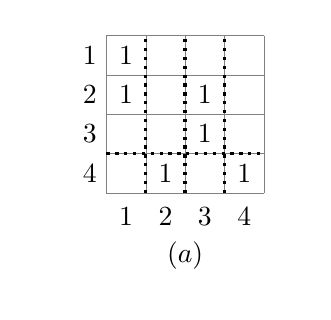
\begin{tikzpicture}
		\coordinate (O) at (0,0);
		
		\clip (-1,-1.25) rectangle (2.5,2.1);
		
		\prgrid{O}{4}{4}
		
		\prvtdline{O}{1}{4};
		
		\prvtdcolumn{O}{1}{4};
		\prvtdcolumn{O}{2}{4};
		\prvtdcolumn{O}{3}{4};
		
		\prbul{O}{1}{2}
		\prbul{O}{1}{4}
		\prbul{O}{2}{3}
		\prbul{O}{3}{1}
		\prbul{O}{3}{3}
		\prbul{O}{4}{1}
		
		
		\draw ($(O)+(-0,0.25)$) node[anchor=east] {$4$};
		\draw ($(O)+(-0,0.75)$) node[anchor=east] {$3$};
		\draw ($(O)+(-0,1.25)$) node[anchor=east] {$2$};
		\draw ($(O)+(-0,1.75)$) node[anchor=east] {$1$};
		
		\draw ($(O)+(0.25,-0.3)$) node {$1$};
		\draw ($(O)+(0.75,-0.3)$) node {$2$};
		\draw ($(O)+(1.25,-0.3)$) node {$3$};
		\draw ($(O)+(1.75,-0.3)$) node {$4$};
		
		\draw ($(O)+(1,-0.8)$) node {$(a)$};
		
	\end{tikzpicture}
	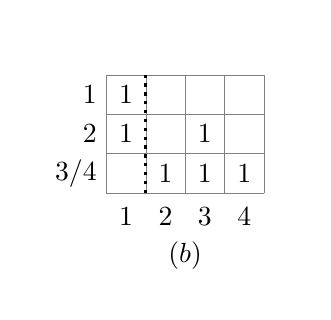
\begin{tikzpicture}
	\coordinate (O) at (0,0);
	
	\clip (-1,-1.25) rectangle (2.5,2.1);
	
	\prgrid{O}{3}{4}
	
	\prbul{O}{1}{2}
	\prbul{O}{1}{3}
	\prbul{O}{1}{4}
	\prbul{O}{2}{1}
	\prbul{O}{2}{3}
	\prbul{O}{3}{1}
		
	\prvtdcolumn{O}{1}{3};
	
	
	\draw ($(O)+(-0,0.25)$) node[anchor=east] {$3/4$};
	\draw ($(O)+(-0,0.75)$) node[anchor=east] {$2$};
	\draw ($(O)+(-0,1.25)$) node[anchor=east] {$1$};
	
	\draw ($(O)+(0.25,-0.3)$) node {$1$};
	\draw ($(O)+(0.75,-0.3)$) node {$2$};
	\draw ($(O)+(1.25,-0.3)$) node {$3$};
	\draw ($(O)+(1.75,-0.3)$) node {$4$};
	\draw ($(O)+(1,-0.8)$) node {$(b)$};
	\end{tikzpicture}
	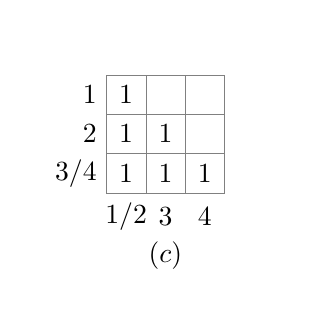
\begin{tikzpicture}
	\coordinate (O) at (0,0);
	
	\clip (-1,-1.25) rectangle (2.5,2.1);
	
	\prgrid{O}{3}{3}
	
	\prbul{O}{1}{1}
	\prbul{O}{1}{2}
	\prbul{O}{1}{3}
	\prbul{O}{2}{1}
	\prbul{O}{2}{2}
	\prbul{O}{3}{1}
	
	
	\draw ($(O)+(-0,0.25)$) node[anchor=east] {$3/4$};
	\draw ($(O)+(-0,0.75)$) node[anchor=east] {$2$};
	\draw ($(O)+(-0,1.25)$) node[anchor=east] {$1$};
	
	\draw ($(O)+(0.25,-0.3)$) node {$1/2$};
	\draw ($(O)+(0.75,-0.3)$) node {$3$};
	\draw ($(O)+(1.25,-0.3)$) node {$4$};
	\draw ($(O)+(0.75,-0.8)$) node {$(c)$};
	
	\end{tikzpicture}
  }
	\caption{In Figure~\ref{fig:introduction:example}.a, we give a $4 \times 4$ grid containing 6 dots. Valid contractions are represented by dotted lines and columns. It is not allowed to contract lines 1 and 2 because the two dots (1;1) and (2;1) would be brought into the same entry. Figure~\ref{fig:introduction:example}.b is the result of the contraction of lines 3 and 4 and Figure~\ref{fig:introduction:example}.c is the contraction of columns 1 and 2. The number of neighbor pairs in each grid is respectively 4, 7 and 10.
  }
	\label{fig:introduction:example}
\end{figure}
\vspace{-0.3cm}



\paragraph{Motivation. }
This problem has an application in optimal sizing of wind-farms \cite{Pillai2015} where we must first define, from a given set of wind-farms location, the neighborhood graph of this set, i.e. the graph such that two wind farms are connected if and only if their corresponding entries in the grid are neighbors. More precisely, given a set of points in the plane, we consider a first grid-embedding such that any two points are at least separated by one vertical line and one horizontal line. Then, we consider the problem of deciding which lines and columns to contract such that the derived embedding maximize the density of the grid, i.e., the number of edges in the corresponding neighbor graph.
\vspace{-0.2cm}
\paragraph{Contributions. } In this paper, we formally define the grid contraction problem as a binary matrix contraction problem in which every dot is a 1 and every other entry is 0. We study the complexity and the polynomial approximability of the problem. Especially, we prove this problem to be NP-Complete. Nonetheless, every algorithm solving this problem is at most a $2\sqrt{n}$-approximation algorithm where $n$ is the number of $1$ in the matrix. We then focus on efficient algorithms to solve the problem. We first investigate the mathematical programming formulation of MMC. We give two formulations: a straightforward non-linear program and a linear program.
Secondly, we describe three polynomial heuristics for the problem. We finally give numerical tests to compare the performances of the linear program and each algorithm. 

In Section~\ref{sec:problemdef}, we give a formal definition of the problem. In Section~\ref{sect:complexity}, we prove that the corresponding decision problem is NP-complete, then we give, in Section~\ref{sect:approx} some results about approximability of the problem. In Section~\ref{sec:linearprog} we derive a linear integer program for the model and run some experiments, then in the next section, we present and compare the three different heuristics.

\section{Problem definition}
\label{sec:problemdef}

The following definitions formalize the problem we want to solve with binary matrices. A binary matrix is a matrix with entries from $\{0,1\}$. Such a matrix modelizes a grid in which each dot is a 1 in the matrix.

\begin{definition}
Let $M$ be a binary matrix with $p$ lines and $q$ columns. For each $I \in \llbracket 1; p-1 \rrbracket$ and each $j \in \llbracket 1; q-1 \rrbracket$, we define the \emph{line contraction matrix} $L_i$ and the \emph{column contraction matrix} $C_j$ by 

$$L_i = \hspace{0.2cm}\begin{blockarray}{ccccccccccccc}
& & & & & & & & & & &\\
\begin{block}{(cccccccccc)ccc}
1      &  0     & \cdots & 0      & 0 & 0 &  0  & 0 & \cdots & 0 &&&\\
0      &  1     & \cdots & 0      & 0 & 0 &  0  & 0 & \cdots & 0 &&&\\
\vdots & \vdots & \ddots & \vdots & \vdots & \vdots &  \vdots  & \vdots & \ddots  & \vdots  &&&\\
0      &   0    &\cdots  & 1      & 0 & 0 &  0  & 0 & \cdots & 0 &&&\\ 
0      &   0    &\cdots  & 0      & 1 & 1 &  0  & 0 & \cdots & 0 & && i\\ 
0      &   0    &\cdots  & 0      & 0 & 0 &  1  & 0 & \cdots & 0 &&&\\
0      &   0    &\cdots  & 0      & 0 & 0 &  0  & 1 & \cdots & 0 &&&\\ 
\vdots      &   \vdots    &\ddots  & \vdots     & \vdots & \vdots & \vdots & \vdots & \ddots & \vdots  &&&\\
0      &   0    &\cdots  & 0      & 0 & 0  &  0 & 0 & \cdots & 1 &&&\\
0      &   0    &\cdots  & 0      & 0 & 0      &   0    & 0      &\cdots  & 0 &&&\\
\end{block}
\end{blockarray}
\hspace{0.5cm}
C_j = \hspace{0.2cm}\begin{blockarray}{ccccccccccc}
 & & & & j & & & & &\\
\begin{block}{(cccccccccc)c}
1      &  0     & \cdots & 0      & 0 & 0 &  0  & \cdots & 0 & 0 &\\
0      &  1     & \cdots & 0      & 0 & 0 &  0  & \cdots & 0 & 0 &\\
\vdots & \vdots & \ddots & \vdots & \vdots & \vdots &  \vdots  & \ddots & \vdots  & \vdots  &\\
0      &   0    &\cdots  & 1      & 0 & 0 &  0  & \cdots & 0 & 0 &\\ 
0      &   0    &\cdots  & 0      & 1 & 0 &  0  & \cdots & 0 & 0 &\\ 
0      &   0    &\cdots  & 0      & 1 & 0 &  0  & \cdots & 0 & 0 &\\
0      &   0    &\cdots  & 0      & 0 & 1 &  0  & \cdots & 0 & 0 &\\ 
0      &   0    &\cdots  & 0      & 0 & 0  &  1 & \cdots & 0 & 0 &\\
\vdots      &   \vdots    &\ddots  & \vdots     & \vdots & \vdots & \vdots & \ddots & \vdots & \vdots  &\\
0      &   0    &\cdots  & 0      & 0 & 0      &   0    &\cdots  & 1      & 0 &\\
\end{block}
\end{blockarray}
$$
\end{definition}

\begin{definition}
Let $M$ be a binary matrix of size $p \times q$, $I = \{i_1, i_2, \dots, i_{|I|}\}$ a sublist of $\llbracket 1;p-1 \rrbracket$ and $J = \{j_1, j_2, \dots, j_{|I|}\}$ a sublist of $\llbracket 1;q-1 \rrbracket$. We assume $I$ and $J$ are sorted. We define the \emph{contraction $C(M,I,J)$ of the lines $I$ and the columns $J$ of $M$} by the following matrix
$$
C(M,I,J) = \left(\prod\limits_{k = 1}^{|I|} L_{i_k}\right) \cdot M \cdot \left(\prod\limits_{k = |J|}^{1} C_{j_k}\right)
$$
\end{definition}

\begin{definition}
	A contraction $C(M,I,J)$ is said \emph{legal} if and only if $C(M,I,J)$ is a binary matrix.
\end{definition}

For example, the contraction of the $j$-th column of a matrix such that $M_{i,j} = M_{i,j+1} = 1$ is not legal because it contains a $2$ at line $i$ and column $j$.

\begin{definition}
	Let $M$ be a binary matrix of size $p \times q$. The \emph{density} is the number of neighbor pairs of 1 in the matrix (including the diagonal pairs). This value may be computed with the following formula :
	$$ 
	d(M) = \frac{1}{2} \cdot \sum\limits_{i,j} \left( M_{i,j} \cdot \left(\sum\limits_{\delta = -1}^1 \sum\limits_{\gamma = -1}^1  M_{i+\delta,j+\gamma}\right) - 1 \right)
	$$
	where we define that $M_{i,j}=0$ if $(i,j) \notin \llbracket 1;p-1 \rrbracket \times \llbracket 1;q-1 \rrbracket$
\end{definition}

\begin{problem}\label{problem1}
	\emph{Maximum Matrix Contraction problem} (MMC). Given a binary matrix $M$ of size $p \times q$ such that $n$ entries equal 1 and $p \cdot q - n$ entries equal 0, the Maximum Matrix Contraction problem consists in the search for two sublists $I$ of $\llbracket 1;p-1 \rrbracket$ and $J$ of $\llbracket 1;q-1 \rrbracket$ such that the contraction $C(M,I,J)$ is legal and maximize $d(C(M,I,J))$.
\end{problem}

We study in the next two sections the complexity and the approximability of this problem.


\section{Complexity}
\label{sect:complexity}
 
This section is dedicated to proving the NP-Completeness of the problem.

  \begin{theorem}
  \label{theo:complexity}
  The decision version of (MMC) is NP-Complete.
  \end{theorem}
  \begin{proof}
 

    Lets $M$ be an instance of MMC. Given an integer $K$, a subset $I$ of $\llbracket 1; p-1 \rrbracket$ and a subset $J$ of $\llbracket 1; q-1 \rrbracket$, one can compute in polynomial time the matrix $C(M,I,J)$ and checks if $d(C(M,I,J)) \geq K$. This proves the problem belongs to NP.

    In order to prove the NP-Hardness, we describe a polynomial reduction from the Maximum Clique problem. Lets $G(V,E)$ be an instance of the Maximum Clique problem, we build an instance $M$ of MMC with $p = q = (4|V| + 6)$. We arbitrarily number the nodes of $G$ : $V = \{v_1, v_2, \dots v_n\}$.

    Let $l_i$ and$c_i$ be respectively the $6+4(i-1)+1$-th line and the $6+4(i-1)+1$-th column. We associate the lines $l_i$ to $l_i+3$ and the columns $c_i$ to $c_i + 3$ to $v_i$. The key idea of the reduction is that each node $v$ is associated with two 1. If we chose the node $v$ to be in the clique, then, firstly, the two 1 it is associated with are moved next to each other and this increases the density by one; and secondly, for every node $w$ such that $(v,w) \not\in E$, the two 1 it is associated to cannot be moved anymore.

    We use three gadgets in this reduction, described in Figure~\ref{fig:reduction:gadgets}. The gadget $(\alpha_i)$ is added at the intersection of the lines and the columns associated with the node $v_i$. The gadget $(\beta_{i,j})$ is added at the intersection of the lines of $v_i$ and the columns of $v_j$ such that $(v_i,v_j) \not\in E$. If $v_i$ and $v_j$ are linked with an edge in $G$, there is no 1 at the intersections of the lines of $v_i$ and the column of $v_j$. We add the gadget $(\gamma_i)$ for each node $v_i$ at line 1, and a symetric gadget at column 1. Finally, we set $M_{1,j} = M_{j,1} = 1$ for each $j \in \llbracket 1;6 \rrbracket$. A complete example is given in Figure~\ref{fig:reduction:example}.

\begin{figure}
\centering
		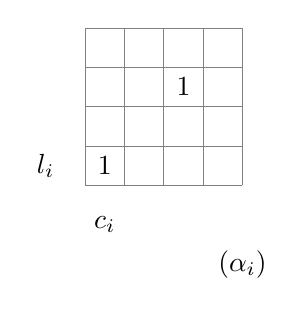
\begin{tikzpicture}
		\coordinate (O) at (0,0);

    \prgrid{O}{4}{4}
    
    \prbul{O}{1}{1}
    \prbul{O}{3}{3}
    \draw ($(O)+(0.25,-0.5)$) node {$c_i$};
    \draw ($(O)+(-0.5,0.25)$) node {$l_i$};
    \draw ($(O)+(2,-1)$) node {$(\alpha_i)$};
    \end{tikzpicture}
		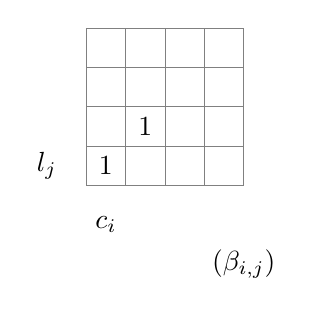
\begin{tikzpicture}
		\coordinate (O) at (0,0);

    \prgrid{O}{4}{4}
    
    \prbul{O}{1}{1}
    \prbul{O}{2}{2}
    \draw ($(O)+(0.25,-0.5)$) node {$c_i$};
    \draw ($(O)+(-0.5,0.25)$) node {$l_j$};
    \draw ($(O)+(2,-1)$) node {$(\beta_{i,j})$};
    \end{tikzpicture}
		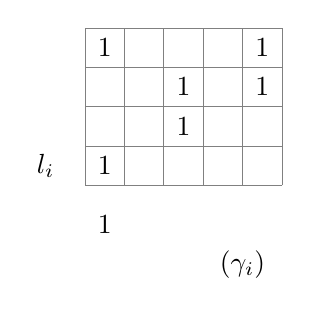
\begin{tikzpicture}
		\coordinate (O) at (0,0);

    \prgrid{O}{4}{5}
    
    \prbul{O}{1}{1};
    \prbul{O}{2}{3};
    \prbul{O}{3}{3};
    \prbul{O}{3}{5};
    \prbul{O}{4}{5};
    \prbul{O}{4}{1};
    
    \draw ($(O)+(0.25,-0.5)$) node {$1$};
    \draw ($(O)+(-0.5,0.25)$) node {$l_i$};
    \draw ($(O)+(2,-1)$) node {$(\gamma_i)$};
    \end{tikzpicture}

\caption{The three gadgets of the reduction. We specify on each gadget the indexes of its lines and columns.}
   \label{fig:reduction:gadgets}
\end{figure}

\begin{figure}
\centering

		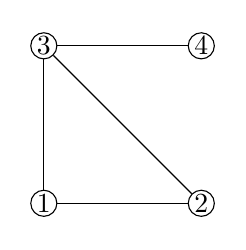
\begin{tikzpicture}
		\tikzset{tinoeud/.style={draw, circle, minimum height=0.1cm}}
		\node[tinoeud] (U) at (0,0) {};
		\node[tinoeud] (V) at (2,0) {};
		\node[tinoeud] (W) at (0,2) {};
		\node[tinoeud] (T) at (2,2) {};

    \draw (U) -- (V);
    \draw (V) -- (W);
    \draw (W) -- (U);
    \draw (W) -- (T);

    \draw (U) node {$1$};
    \draw (V) node {$2$};
    \draw (W) node {$3$};
    \draw (T) node {$4$};

		\end{tikzpicture}

		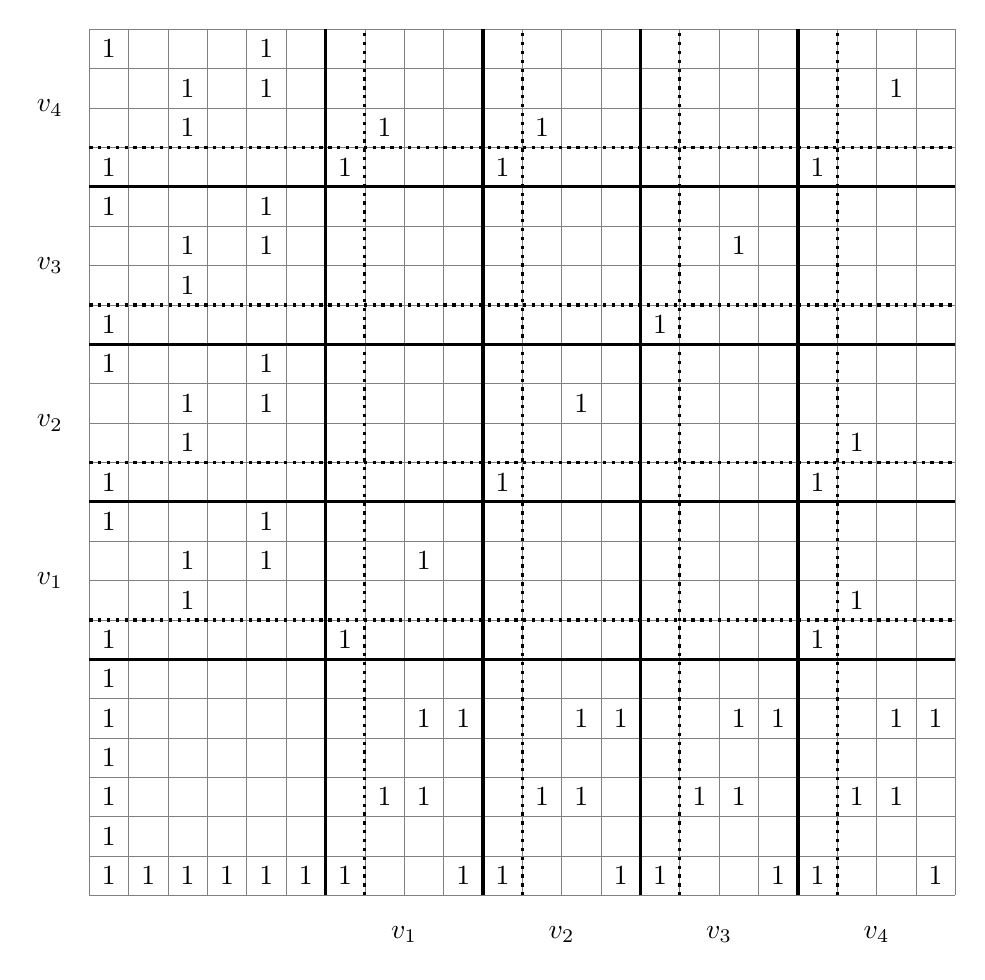
\begin{tikzpicture}
		
		\coordinate (O) at (0,0);

    \prgrid{O}{22}{22}

    \prvtline{O}{6}{22}
    \prvtline{O}{10}{22}
    \prvtline{O}{14}{22}
    \prvtline{O}{18}{22}
    
    \prvtcolumn{O}{6}{22}
    \prvtcolumn{O}{10}{22}
    \prvtcolumn{O}{14}{22}
    \prvtcolumn{O}{18}{22}
    
    \prvtdline{O}{7}{22}
    \prvtdline{O}{11}{22}
    \prvtdline{O}{15}{22}
    \prvtdline{O}{19}{22}
    
    \prvtdcolumn{O}{7}{22}
    \prvtdcolumn{O}{11}{22}
    \prvtdcolumn{O}{15}{22}
    \prvtdcolumn{O}{19}{22}
    
    \draw ($(O)+(-0.5,4)$) node {$v_1$};
    \draw ($(O)+(-0.5,6)$) node {$v_2$};
    \draw ($(O)+(-0.5,8)$) node {$v_3$};
    \draw ($(O)+(-0.5,10)$) node {$v_4$};
    
    \draw ($(O)+(4,-0.5)$) node {$v_1$};
    \draw ($(O)+(6,-0.5)$) node {$v_2$};
    \draw ($(O)+(8,-0.5)$) node {$v_3$};
    \draw ($(O)+(10,-0.5)$) node {$v_4$};

    \prbul{O}{1}{1};
    \prbul{O}{1}{2};
    \prbul{O}{1}{3};
    \prbul{O}{1}{4};
    \prbul{O}{1}{5};
    \prbul{O}{1}{6};
    
    \prbul{O}{2}{1};
    \prbul{O}{3}{1};
    \prbul{O}{4}{1};
    \prbul{O}{5}{1};
    \prbul{O}{6}{1};
 
    \prbul{O}{7}{1};
    \prbul{O}{8}{3};
    \prbul{O}{9}{3};
    \prbul{O}{9}{5};
    \prbul{O}{10}{5};
    \prbul{O}{10}{1};
 
    \prbul{O}{11}{1};
    \prbul{O}{12}{3};
    \prbul{O}{13}{3};
    \prbul{O}{13}{5};
    \prbul{O}{14}{5};
    \prbul{O}{14}{1};
 
    \prbul{O}{15}{1};
    \prbul{O}{16}{3};
    \prbul{O}{17}{3};
    \prbul{O}{17}{5};
    \prbul{O}{18}{5};
    \prbul{O}{18}{1};
 
    \prbul{O}{19}{1};
    \prbul{O}{20}{3};
    \prbul{O}{21}{3};
    \prbul{O}{21}{5};
    \prbul{O}{22}{5};
    \prbul{O}{22}{1};
		
 
    \prbul{O}{1}{7};
    \prbul{O}{3}{8};
    \prbul{O}{3}{9};
    \prbul{O}{5}{9};
    \prbul{O}{5}{10};
    \prbul{O}{1}{10};
 
    \prbul{O}{1}{11};
    \prbul{O}{3}{12};
    \prbul{O}{3}{13};
    \prbul{O}{5}{13};
    \prbul{O}{5}{14};
    \prbul{O}{1}{14};
 
    \prbul{O}{1}{15};
    \prbul{O}{3}{16};
    \prbul{O}{3}{17};
    \prbul{O}{5}{17};
    \prbul{O}{5}{18};
    \prbul{O}{1}{18};
 
    \prbul{O}{1}{19};
    \prbul{O}{3}{20};
    \prbul{O}{3}{21};
    \prbul{O}{5}{21};
    \prbul{O}{5}{22};
    \prbul{O}{1}{22};


    \prbul{O}{7}{7};
    \prbul{O}{9}{9};

    \prbul{O}{11}{11};
    \prbul{O}{13}{13};

    \prbul{O}{15}{15};
    \prbul{O}{17}{17};

    \prbul{O}{19}{19};
    \prbul{O}{21}{21};


    \prbul{O}{7}{19};
    \prbul{O}{8}{20};

    \prbul{O}{19}{7};
    \prbul{O}{20}{8};

    \prbul{O}{11}{19};
    \prbul{O}{12}{20};

    \prbul{O}{19}{11};
    \prbul{O}{20}{12};

  
    \end{tikzpicture}

\caption{This figure illustrates, on the first part, a graph in which we search for a maximum clique and, on the second part, the matrix obtained built with the reduction.}
\label{fig:reduction:example}
\end{figure}

The initial density in this matrix is $d_0 = 11 + 6|V| + (|V| (|V|-1) - 2|E|)$. Note that, firstly, only the lines $l_i$ and columns $c_i$ for $i \in \llbracket 1;n \rrbracket$ may be contracted and, secondly, we cannot increase the density of the 1's that are not contained in the gadgets $(a_i)$. In order to add one to the density of the matrix we must choose a node $v_i$ and contract the column $c_i$ and the line $l_i$. 

If the column $c_i$ is contracted and if $(v_i, v_j) \not \in E$, the two 1's of the gadget $(\beta_{i,j})$ are moved on the same column. Similarly, if the line $l_i$ is contracted, the two 1's of the gadget $(\beta_{j,i})$ are moved on the same column. This prohibits the contraction of the line $l_j$ and thecolumn $c_j$. Consequently, in order to add $C$ to the density, we must find a clique of size $C$ in the graph and contract every line and column associated with the nodes of that clique.

Thus, there is a clique of size $K$ if and only if there is a feasible solution for $M$ of density $d_0 + K$. This concludes the proof of NP-Completeness.

  \end{proof}

\section{Approximability}
\label{sect:approx}

In this section we define the notion of maximal feasible solution and prove that every algorithm returning a maximal feasible solution is a $2\sqrt{n}$ approximation.

\begin{definition}
We say a feasible solution is \emph{maximal} if it is not strictly included in another feasible solution. In oher words, when all the lines and columns of that solution are contracted, it is not possible to legally contract any other line or column.
\end{definition}

\begin{lemma}
\label{lem:bounds}
Let $M$ be an instance of MMC, $(I,J)$ be a maximal feasible solution and $M' = C(M,I,J)$ then $2 \sqrt{n} \leq d(M') \leq 4n$.
\end{lemma}
\begin{proof}
A 1 in a matrix cannot have more than $8$ neighbors, thus the density of $M'$ is no more than $4n$.

For each two lines $i$ and $i+1$ of $M'$, there is a column $j$ such that $M'_{i,j} = M'_{i+1,j} = 1$ otherwise we could contract line $i$ and $(I,J)$ would not be maximal. Similarly for each column $j$. Thus $d(M') \geq p'+q'$ where $p'$ and $q'$ are respectively the number of lines and columns of $M'$.

\begin{align*}
\intertext{From the inequality of arithmetic and geometric means}
p' + q ' &\geq 2 \sqrt{p'\cdot q'}
\intertext{As $M'$ contains $n$ 1's, $p'\cdot q' \geq n$}
p' + q ' &\geq 2 \sqrt{n}
\end{align*}
\end{proof}

From the upper bound and the lower bound given in the previous lemma, we can immediately prove the following theorem. 

\begin{theorem}
	\label{theo:sqrtnapprox}
An algorithm returning any maximal solution of an instance of MMC is a $2\sqrt{n}$-approximation.
\end{theorem}

Theorem~\ref{theo:sqrtnapprox} proves a default ratio for every algorithm trying to solve the problem. Note that there are instances in which the ratio between an optimal density and the lowest density of a maximal solution is $\sqrt{n}$. An example is given in Figure~\ref{fig:badinstance}. In Section~\ref{sect:heuristics}, we describe three natural heuristics to solve the problem. For two of them returns, the instance of Figure~\ref{fig:badinstance} may be adapted to show their approximability ratio is $\sqrt{n}$. 


\begin{figure}
	
		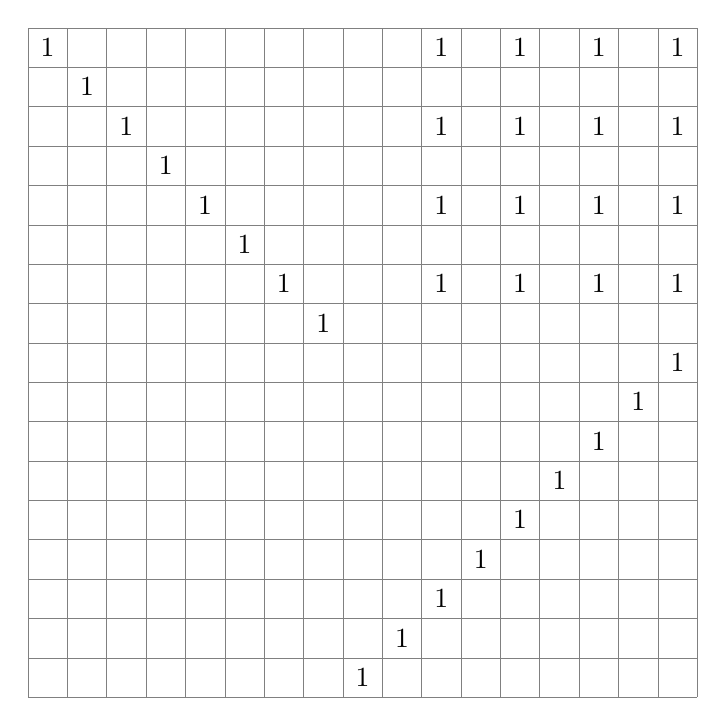
\begin{tikzpicture}
		
		\coordinate (O) at (0,0);

    \prgrid{O}{17}{17}

    \prbul{O}{1}{9};
    \prbul{O}{2}{10};
    \prbul{O}{3}{11};
    \prbul{O}{4}{12};
    \prbul{O}{5}{13};
    \prbul{O}{6}{14};
    \prbul{O}{7}{15};
    \prbul{O}{8}{16};
    \prbul{O}{9}{17};
    
    \prbul{O}{17}{1};
    \prbul{O}{16}{2};
    \prbul{O}{15}{3};
    \prbul{O}{14}{4};
    \prbul{O}{13}{5};
    \prbul{O}{12}{6};
    \prbul{O}{11}{7};
    \prbul{O}{10}{8};
    
    
    \prbul{O}{11}{11};
    \prbul{O}{13}{11};
    \prbul{O}{15}{11};
    \prbul{O}{17}{11};

    \prbul{O}{11}{13};
    \prbul{O}{13}{13};
    \prbul{O}{15}{13};
    \prbul{O}{17}{13};
    
    \prbul{O}{11}{15};
    \prbul{O}{13}{15};
    \prbul{O}{15}{15};
    \prbul{O}{17}{15};
  
    \prbul{O}{11}{17};
    \prbul{O}{13}{17};
    \prbul{O}{15}{17};
    \prbul{O}{17}{17};
    \end{tikzpicture}
		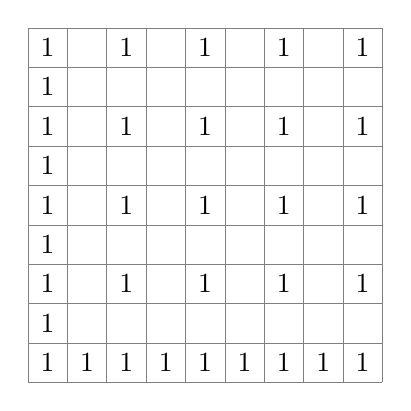
\begin{tikzpicture}
		
		\coordinate (O) at (0,0);

    \prgrid{O}{9}{9}

    \prbul{O}{1}{1};
    \prbul{O}{2}{1};
    \prbul{O}{3}{1};
    \prbul{O}{4}{1};
    \prbul{O}{5}{1};
    \prbul{O}{6}{1};
    \prbul{O}{7}{1};
    \prbul{O}{8}{1};
    \prbul{O}{9}{1};
    
    \prbul{O}{1}{2};
    \prbul{O}{1}{3};
    \prbul{O}{1}{4};
    \prbul{O}{1}{5};
    \prbul{O}{1}{6};
    \prbul{O}{1}{7};
    \prbul{O}{1}{8};
    \prbul{O}{1}{9};

    \prbul{O}{3}{3};
    \prbul{O}{5}{3};
    \prbul{O}{7}{3};
    \prbul{O}{9}{3};
    
    \prbul{O}{3}{5};
    \prbul{O}{5}{5};
    \prbul{O}{7}{5};
    \prbul{O}{9}{5};
  
    \prbul{O}{3}{7};
    \prbul{O}{5}{7};
    \prbul{O}{7}{7};
    \prbul{O}{9}{7};

    \prbul{O}{3}{9};
    \prbul{O}{5}{9};
    \prbul{O}{7}{9};
    \prbul{O}{9}{9};
    \end{tikzpicture}
		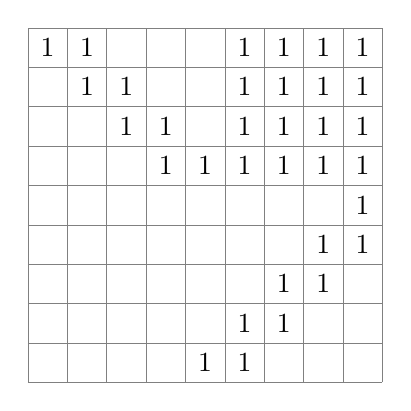
\begin{tikzpicture}
		
		\coordinate (O) at (0,0);

    \prgrid{O}{9}{9}

    \prbul{O}{1}{5};
    \prbul{O}{1}{6};
    \prbul{O}{2}{6};
    \prbul{O}{2}{7};
    \prbul{O}{3}{7};
    \prbul{O}{3}{8};
    \prbul{O}{4}{8};
    \prbul{O}{4}{9};
    \prbul{O}{5}{9};
    
    \prbul{O}{9}{1};
    \prbul{O}{9}{2};
    \prbul{O}{8}{2};
    \prbul{O}{8}{3};
    \prbul{O}{7}{3};
    \prbul{O}{7}{4};
    \prbul{O}{6}{4};
    \prbul{O}{6}{5};
    
    \prbul{O}{6}{6};
    \prbul{O}{7}{6};
    \prbul{O}{8}{6};
    \prbul{O}{9}{6};
    
    \prbul{O}{6}{7};
    \prbul{O}{7}{7};
    \prbul{O}{8}{7};
    \prbul{O}{9}{7};

    \prbul{O}{6}{8};
    \prbul{O}{7}{8};
    \prbul{O}{8}{8};
    \prbul{O}{9}{8};

    \prbul{O}{6}{9};
    \prbul{O}{7}{9};
    \prbul{O}{8}{9};
    \prbul{O}{9}{9};
    \end{tikzpicture}
\caption{In this instance, the density of an optimal solution is $O(n)$ and there is a maximal solution of density $O(\sqrt{n})$.}

\label{fig:badinstance}
  \end{figure}
  
  \begin{comment}
  Il faudra probablement mettre cette figure en annexe.
  \end{comment}

Determining if MMC can be approximated to within a constant factor is an open question. As it was already pointed at the end of section~\ref{sect:complexity}, the problem may possibly be not approximable to within $n^{\frac{1}{2}-\varepsilon}$ and this would almost tight the approximability of MMC.

The next two sections focus on efficient algorithms to solve the problem. The next section is dedicated to the mathematical programming methods.

\section{Linear programming}\label{sec:linearprog}

For $i \in \llbracket 1; p-1 \rrbracket$ (resp.  $j \in \llbracket 1; q-1 \rrbracket$ ), let $x_i$ (resp> $y_j$) be the binary variable such that $x_i=1$ (resp. $y_j=1$) if and only if line $i$ is contracted, i.e. $i \in I$ (resp. column $j$ is contracted, i.e. $j \in J$). From the definition of \ref{problem1}, we can model the MMC problem by the following non-linear binary program:

\begin{equation*}
(\ast)\left\{
\begin{array}{lll}
\max\limits_{x,y} & \quad	d(A)  \\
& A= \prod\limits_{i=0}^{p-1}
\end{array}\right.
\end{equation*}
where we recall that $$= \frac{1}{2} \cdot \sum\limits_{i,j} \left( M_{i,j} \cdot \left(\sum\limits_{\delta = -1}^1 \sum\limits_{\gamma = -1}^1  M_{i+\delta,j+\gamma}\right) - 1 \right)$$

\begin{comment}
\begin{itemize}
\item Si c'est pas fait dans la section 2, présenter le programme non linéaire et expliquer pourquoi il ne peut être linéarisé tel quel
\item Présentation de la version temporisée
\item Remarque sur la exactitude du programme
\end{itemize}
\end{comment}

\subsection{Numerical results}

\todo{Tester, mettre sous forme de tableau, commenter.}


\section{Heuristics}

\begin{comment}
\begin{itemize}
\item Avant toute chose tester Greedy VS LCL VS Neighborization sur des grosses instances (jusqu'à combien va le LCL?).
\item Présenter ceux qui marchent et ceux qui marchent pas
\item Contreexemple? Explication rapide du pire cas?
\end{itemize}
\end{comment}

This section is dedicated to describing a simple and fast heuristic. Note that this heuristic is, in the worst case, a $2\sqrt{n}$-approximation.

The LCL algorithm is divided into two parts : the LC (Line Column) part and the CL (Column Line) part. The LC computes and return a maximal feasible solution $M^{LC}$ by contracting a maximal set of lines $I^{LC}$ and, then, by contracting a maximal set of columns $J^{LC}$. The CL part computes and returns a maximal feasible solution $M^{CL}$ by starting with the columns and ending with the lines. The LCL algorithm then returns the solution with the maximum density.


\subsection{Numerical results}

\todo{Tester, mettre sous forme de tableau, commenter.}


\section{Conclusion}

\todo{Faire la conclusion}


\bibliographystyle{splncs}
\bibliography{edla}

\end{document}
